\documentclass[english]{article}
\usepackage[round]{natbib} 
\usepackage{listings}

\bibliographystyle{abbrvnat}
%\usepackage{thumbpdf}
\usepackage{hyperref}

\linespread{2.0} 
 
\usepackage{Sweave}
\begin{document}


\Sconcordance{concordance:statTarget.tex:statTarget.Rnw:%
1 6 1 1 0 92 1 1 2 5 0 1 2 1 4 2 1}


\author{Hemi Luan}

\title{statTarget:\\Statistical Analysis of Metabolite Profile}
%\VignetteIndexEntry{Introduction to statTarget}


\maketitle

\tableofcontents
 
\newpage

\section{Background}

Quality Control (QC) has been considered as an essential step in the
metabolomics platform for high reproducibility and accuracy of data. 
The secondary use of the same QC samples is more and more acceptable for 
correcting the signal drift during the sequence of MS run order, 
especially benefiting to improve the quality of data in multi-block 
experiments of large-scale metabolomic study. statTarget is easy use tool 
to provide a graphical user interface for quality control based 
shift signal correction, integration of metabolomic data from multi-batch 
experiments, and the comprehensive statistic analysis in 
non-targeted or targeted metabolomics.
This document is intended to guide the user to use statTargetGUI to 
perform metabolomic data analysis. Note that this document will 
not describe the inner workings 
of statTarget algorithm.

\subsection{System requirements}

Dependent on R (>= 3.3.0)


\subsection{Opening the GUI}
 
Load the package with biocLite():

source("https://bioconductor.org/biocLite.R")

biocLite("statTarget")

**For mac PC, the package "statTargetGUI" requires X11 support (XQuartz). 
Download it from https://www.xquartz.org.

\newpage 

\section[GUI overview]{GUI overview}
 

An easy to use tool provide a graphical user interface (Figure 1) for 
quality control based signal correction, integration of metabolomic 
data from multiple batches, and the comprehensive statistic analysis 
for non-targeted and targeted approaches. 
(URL: \url{https://github.com/13479776/statTarget})

\subsection[What does statTarget offer statistically]{
What does statTarget offer statistically}


The main GUI of statTarget has two basic components. The first components 
is shift correction. It includes quality control-based robust LOESS signal 
correction (QC-RLSC) that is a widely accepted method for quality control 
based signal correction and integration of metabolomic data from multiple 
analytical batches (Dunn WB., et al. 2011; Luan H., et al. 2015). The second 
components is Statistical Analysis. It provides comprehensively computational 
and statistical methods that are commonly applied to analyze metabolomics data,
and offers multiple results for biomarker discovery.


\begin{figure}

\centering

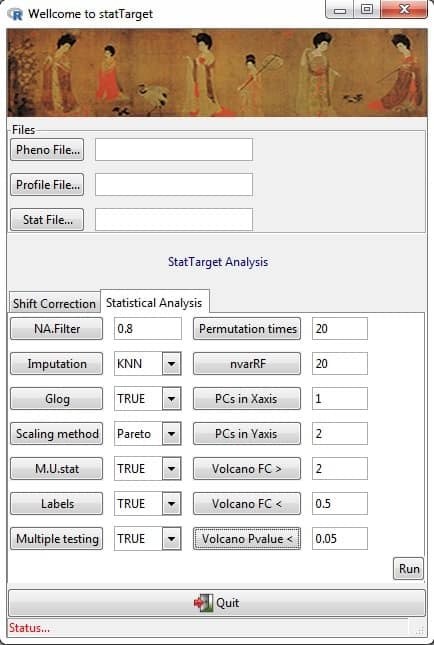
\includegraphics[width=2.5in]{statTarget}

\caption{\label{fig:statTarget}The main GUI of statTarget}

\end{figure}


\subsection[Primary functions of statTarget]{Primary functions of statTarget}


 
\textbf{Function 1 - Shift Correction} provide QC-RLSC algorithm 
that fit the QC data, 
and each metabolites in the true sample will be normalized to the QC sample.
To avoid overfitting of the observed data, LOESS based generalised 
cross-validation (GCV) would be automatically applied, 
when the QCspan was set at 0. 




\textbf{Function 2 - Statistical Analysis} provide features including Data preprocessing,
Data descriptions, Multivariate statistics analysis and Univariate analysis.


Data preprocessing : 80-precent rule, log transformation, KNN imputation, 
Median imputation and Minimum values imputation.


Data descriptions :  Mean value, Median value, Sum, Quartile, Standard 
derivatives, etc.


Multivariate statistics analysis : PCA, PLSDA, VIP, Random forest.


Univariate analysis : Student T-test, Shapiro-Wilk normality test and 
Mann-Whitney test.


Biomarkers analysis: ROC, Odd ratio.


\section[Running Shift Correction from the GUI]{
Running Shift Correction from the GUI}




\textbf{Pheno File}
  
  
  Meta information includes the Sample name, class, batch and order. 
  Do not change the name of each column. 
  (a) Class: The QC should be labeled as NA. 
  (b) Order : Injection sequence. 
  (c) Batch: The analysis blocks or batches with ordinal number,e.g., 1,2,3,.... 
  (d) Sample name should be consistent in Pheno file and Profile file. 
  (See the example data)


\textbf{Profile File}


Expression data includes the sample name and expression
data.(See the example data)


\textbf{NA.Filter}


 NA.Filter: Removing peaks with more than 80 percent of missing values
 (NA or 0) in each group. (Default: 0.8) 


\textbf{QCspan}


The smoothing parameter which controls the bias-variance tradeoff. 
The common range of QCspan value is from 0.2 to 0.75. If you choose
a span that is too small then there will be a large variance. 
If the span is too large, a large bias will be produced. 
The default value of QCspan is set at '0', the generalised 
cross-validation will be performed for choosing a good value, 
avoiding overfitting the observed data. (Default: 0) 


\textbf{degree}


Lets you specify local constant regression (i.e., 
the Nadaraya-Watson estimator, degree=0), 
local linear regression (degree=1), or local polynomial fits (degree=2). 
(Default: 2) 


\textbf{Imputation}


Imputation: The parameter for imputation method.(i.e., 
nearest neighbor averaging, "KNN"; minimum values for imputed variables, 
"min"; median values for imputed variables (Group dependent) "median". 
(Default: KNN) 
 


\section[Running Statistical Analysis from the GUI]{
Running Statistical Analysis from the GUI}


\textbf{Stat File}


Expression data includes the sample name, group, and expression data.


\textbf{NA.Filter}


Removing peaks with more than 80 percent of missing values (NA or 0) 
in each group. (Default: 0.8) 


\textbf{Imputation}


The parameter for imputation method.(i.e., nearest neighbor averaging, 
"KNN"; minimum values for imputed variables, "min";
median values for imputed variables (Group dependent) "median". (Default: KNN)


\textbf{Glog}


Generalised logarithm (glog) transformation for Variance stabilization  
(Default: TRUE)


\textbf{Scaling Method}


Scaling method before statistic analysis (PCA or PLS). 
Pareto can be used for specifying the Pareto scaling. 
Auto can be used for specifying the Auto scaling (or unit variance scaling). 
Vast can be used for specifying the vast scaling. Range can be used for 
specifying the Range scaling. (Default: Pareto) 


\textbf{M.U.Stat}


Multiple statistical analysis and univariate analysis (Default: TRUE) 


\textbf{Permutation times}


The number of random permutation times for PLS-DA model (Default: 20) 



\textbf{PCs}


PCs in the Xaxis or Yaxis: Principal components in 
PCA-PLS model for the x or y-axis (Default: 1 and 2) 


\textbf{nvarRF}


The number of variables in Gini plot of Randomforest model (=< 100).
(Default: 20) 


\textbf{Labels}


To show the name of sample in the Score plot. (Default: TRUE) 


\textbf{Multiple testing}


This multiple testing correction via false discovery rate (FDR) 
estimation with Benjamini-Hochberg method. The false discovery rate 
for conceptualizing the rate of type I errors in null hypothesis 
testing when conducting multiple comparisons. (Default: TRUE) 



\textbf{Volcano FC}


The up or down -regulated metabolites using Fold Changes cut off 
values in the Volcano plot. (Default:  > 2 or < 1.5) 


\textbf{Volcano Pvalue}


The significance level for metabolites in the Volcano plot.(Default: 0.05) 



\section[Investigating the results]{
Investigating the results}

Once data  files have been analysed it is time to investigate them. 
Please get this info. through the GitHub page.
(URL: \url{https://github.com/13479776/statTarget})


 
 
\section[References]{References}

\noindent Dunn, W.B., et al.,Procedures for large-scale metabolic profiling of
serum and plasma using gas chromatography and liquid chromatography coupled 
to mass spectrometry. Nature Protocols 2011, 6, 1060.

\noindent Luan H., LC-MS-Based Urinary Metabolite Signatures in Idiopathic 
Parkinson's Disease. J Proteome Res., 2015, 14,467.

\noindent Luan H., Non-targeted metabolomics and lipidomics LC-MS data 
from maternal plasma of 180 healthy pregnant women. GigaScience 2015 4:16




\section{Session Info}

\begin{itemize}\raggedright
  \item R version 3.3.0 (2016-05-03), \verb|x86_64-apple-darwin13.4.0|
  \item Locale: \verb|en_US.UTF-8/en_US.UTF-8/en_US.UTF-8/C/en_US.UTF-8/en_US.UTF-8|
  \item Base packages: base, datasets, graphics, grDevices, methods, stats, utils
  \item Other packages: devtools~1.11.1, digest~0.6.9, gWidgets2~1.0-7,
    gWidgets2RGtk2~1.0-5, memoise~1.0.0, RGtk2~2.20.31, statTarget~1.2.6
  \item Loaded via a namespace (and not attached): BiocInstaller~1.22.3, cluster~2.0.4,
    DEoptimR~1.0-4, grid~3.3.0, impute~1.46.0, lattice~0.20-33, magrittr~1.5,
    mvtnorm~1.0-5, pcaPP~1.9-60, pdist~1.2, pls~2.5-0, plyr~1.8.3, pROC~1.8,
    randomForest~4.6-12, Rcpp~0.12.4, robustbase~0.92-6, roxygen2~5.0.1, rrcov~1.3-11,
    stats4~3.3.0, stringi~1.0-1, stringr~1.0.0, tools~3.3.0, withr~1.0.1
\end{itemize}


\end{document}
